%!TEX root = ../report.tex

% 
% Evaluation
% 

\section{Evaluation}
\label{Evaluation}

This works validation involves the development of a proof of concept (POC) to prove its usability and claims. This concept will storage organizations data, calculate correspondent KPIs and display it through several graphics. It also creates a raking between the different organizations FM results. 
In order to validate the proposed solution, will be performed a set of tests:

\begin{description}
	\item [Usability Tests] evaluates the application by testing it with users. It provides a direct perception how the users interact with the application, the common errors they make and if they can execute the tasks. As a result of this test, we can understand if the application interface is well designed and perceptible.\\

	\item [Qualitative Tests] combined with the usability tests, are possible to gather users opinions. They can help find better ways to improve the application interface.\\

	\item [Indicators Rating] is very important to realize which indicators are the most convenient to any specific users. This can be achieved by a questionnaire or by integrating an indicator rating tool inside the application, where the users can select their preferable indicators.\\

	\item [Performance Tests] in order to test the cache efficiency on the database. Will be made two tests. For the first test, KPIs will be asked directly to the Input Data Staging Area, on the second test, it will be used a cache, and the KPIs will be asked to the KPI Aggregated Data. This way, it is possible to understand the performance optimization brought by the cache. 
\end{description}

%It will be used a web frameworks and a public or private cloud provider.

%Finally, this work evaluation concludes by inquiring industry organizations through an online survey, to validate this work claims and solution proposal. It’s expected that this validation can prove the claims and conclusions of this work and enhance it credibility.

\subsection{Deployment}
To provide a real situation evaluation and benchmarking, this POC will be deployed on the cloud provider Heroku. Heroku is a PaaS which provides SQL Postgres Database and a Github integration, which permits a quicker and easier deployment of the application while allowing vertical and horizontal scalability on the fly \cite{Heroku}. 


\section{Planning}
\label{Planning}

This document project will follow the methodology depicted on the Gantt Chart of the Figure \ref{fig:PlaneamentoTese}, which can be seen an overall view of the time line of this thesis work.

\begin{figure}[h!]
  \centering
  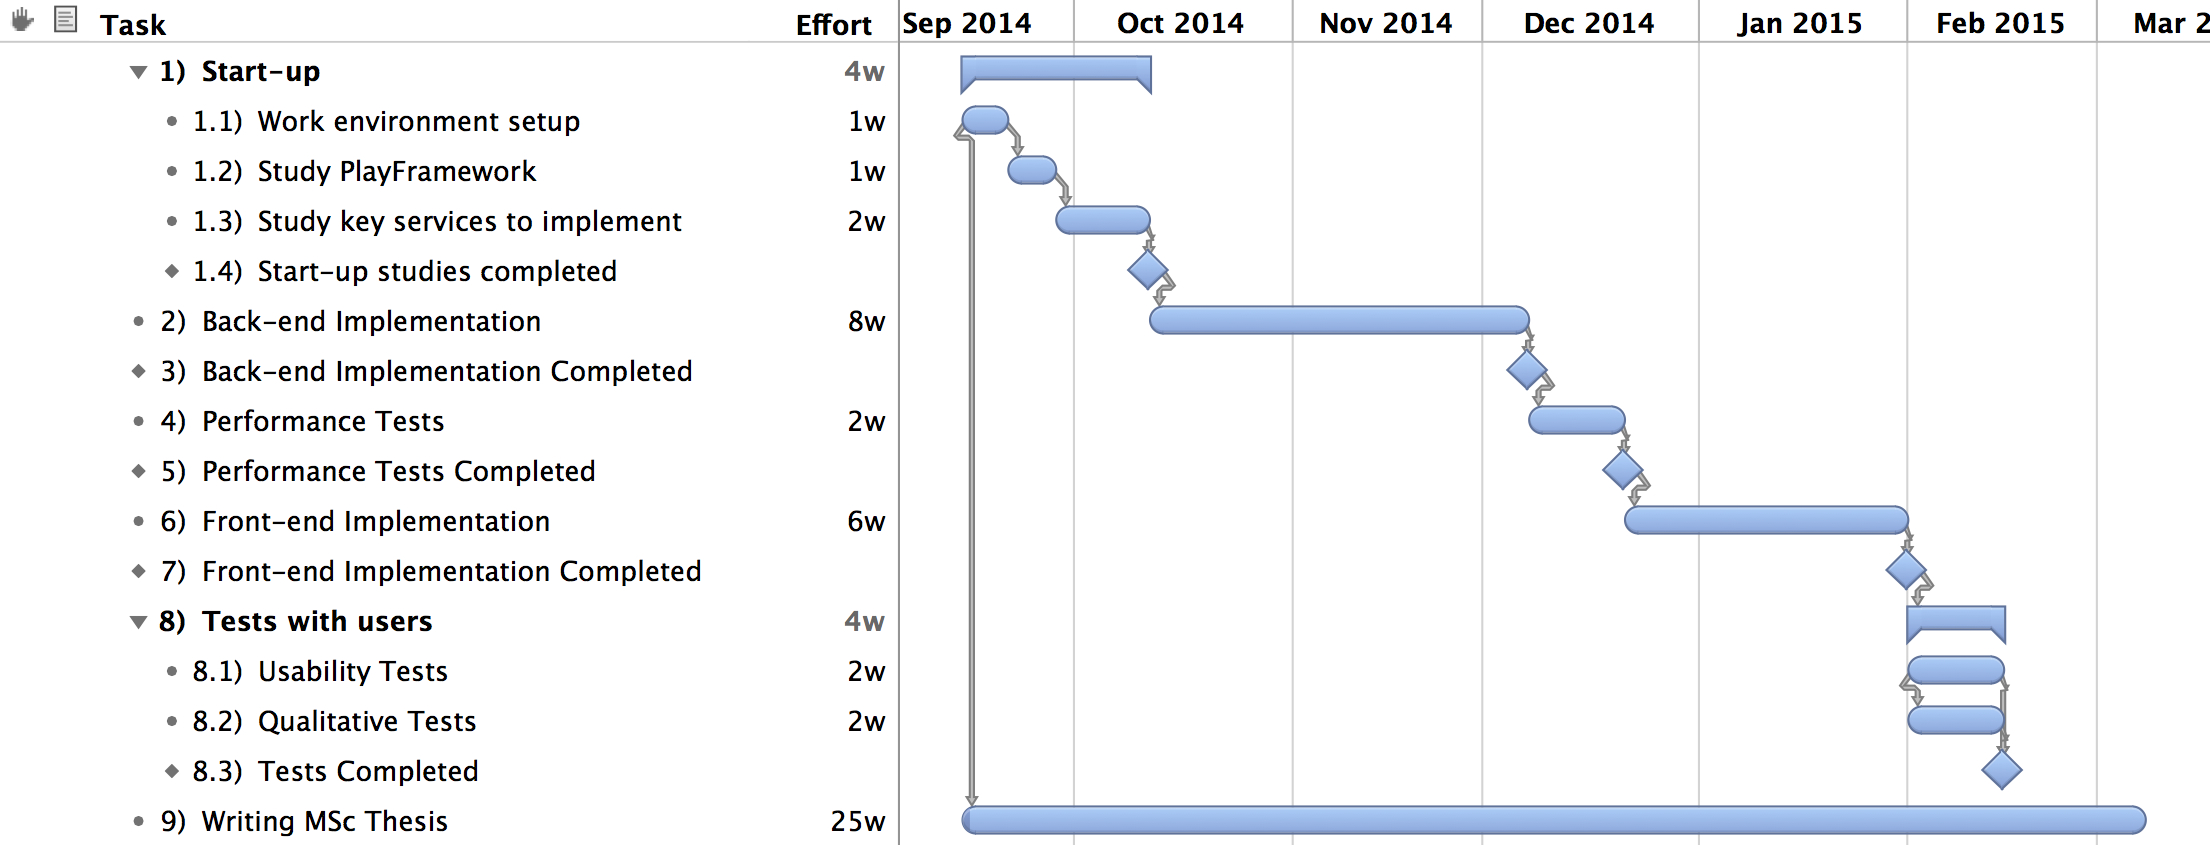
\includegraphics[width=1\textwidth]{img/PlaneamentoTese.jpg}
  \caption{Project Gantt Chart. Task planning and working time estimation.}
  \label{fig:PlaneamentoTese}
\end{figure}


